\chapter{Interazione radiazione-materia}
\section{Interazione tra particelle cariche pesanti e materia}
L'interazione delle particelle cariche pesanti con la materia avviene attraverso una cessione graduale di energia agli elettroni,
Questo comporta una eccitazione o ionizzazione di atomi; un parametro di particolare importanza \`e la \textbf{ionizzazione specifica}:
essa indica la quantit\`a di ionizzazione prodotta per unit\`a di lunghezza.
Nota l'energia media necessaria per produrre ionizzazione in un materiale e la ionizzazione media per unit\`a di lunghezza, \`e possibile legare questo parametro al \textbf{potere frenante}:
\begin{equation*}
S = \left \langle \frac{dE}{dx}\right \rangle
\end{equation*}
Viene, inoltre, definito il \textbf{raggio} (\textit{range}) come il tratto di materiale attraversato fino all'arresto e il
\textbf{raggio medio} come il \textit{range} attraversato dalla met\`a delle particelle ad una data energia.
Per via delle fluttuazioni nella cessione dell'energia alcune particelle percorrono un percorso pi\`u lungo di altre, per questo
si parla di \textbf{raggio estrapolato} come il raggio ottenuto estrapolando il percorso dalla pendenza della curva di \textit{range}
nel punto di raggio medio.
La differenza tra i due raggi viene definita \textbf{\textit{straggling}}.\\
\subsection{La formula di Bethe-Bloch}
La perdita di energia delle particelle cariche pesanti nella materia pu\`o essere descritta dalla \textbf{formula di Bethe-Bloch}:
\begin{equation*}
\frac{S_{\text{coll}}}{\rho} = 4 \, \pi \, r_e^2 \, mc^2 \, N_A \, \frac{Z_m}{A} \, \frac{Z^2}{\beta^2}\left \{ \text{log} \left[ \frac{2 mc^2 \, \beta^2}{I(1-\beta^2)} \right] - \beta^2 \right\}
\end{equation*}
In particolare la formula descrive il \textbf{potere frenante massico}: $\rho$ indica la densit\`a, $r_e$ \`e il \textbf{raggio classico dell'elettrone}, $Z_m$ lo Z del materiale, $Z$ il numero atomico del proiettile e $I$ l'energia media di ionizzazione.
Si pu\`o notare che la formula presenta una debole dipendenza dal materiale, in quanto il rapporto tra Z e A vale circa $0.5$ per molti materiali.
\`E fondamentale notare la presenza di un minimo, ad energia relativistica, una particella con un energia dello stesso ordine del minimo viene detta \textbf{particella a minimo di ionizzazione}
(\textit{minimum ionizing particle} (M.I.P.)).
Ad alte energie si osserva un aumento dell'energia persa, questo \`e dovuto all'emissione di bremsstrahlung.
\section{Interazione tra elettroni e materia}
A differenza delle particelle pesanti, per gli elettroni ha poco senso parlare di cammino medio, in quanto essendo leggeri vengono
fortemente deviati dalle loro interazioni, subendo a volte del \textit{backscattering}.
Per questo motivo parla piuttosto di una distanza di penetrazione media, detta \textbf{percorso pratico o estrapolato}:
\begin{figure}[htbp]
\begin{center}
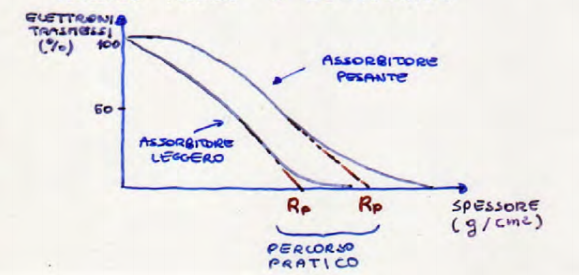
\includegraphics[scale=1]{./Immagini/RangeElettroni.png}
\caption{Percorso pratico degli elettroni}
\end{center}
\end{figure}
Inoltre \`e utilizzato il parametro $\eta$:
\begin{equation*}
\eta = \frac{\# \text{elettroni retrodiffusi}}{\# \text{elettroni incidenti}}
\end{equation*}
Per via della piccola massa degli elettroni, le interazioni con i nuclei sono fondamentali: possiamo osservare scattering multipli e perdite per irraggiamento.\\
Quest'ultimo diventa predominante a energie relativistiche, in particolare le dipendenze \textit{non relativistiche} sono:
\begin{gather*}
S_{coll} \propto \frac{1}{E_k} \, \frac{Z}{A}\\
S_{irr} \propto \frac{Z^2}{A}
\end{gather*}
mentre ad energie relativistiche diventano:
\begin{gather*}
S_{coll} \propto \frac{Z}{A}\\
S_{irr} \propto \frac{Z^2}{A}\, E_k
\end{gather*}
Si definisce \textbf{energia critica}, il valore dell'energia cinetica per cui le due $S$ si equivalgono, esso vale circa:
\begin{equation*}
E_c = \frac{550}{Z} \text{MeV}
\end{equation*}
da cui si deduce che nei materiali pesanti l'irraggiamento diventa prevalente ad energie pi\`u basse.\\
Un parametro fondamentale \`e la \textbf{lunghezza di radiazione}:
\begin{equation*}
X_0 \approx 170 \frac{A}{Z^2} \frac{\text{g}}{\text{cm}^2}
\end{equation*}
Essa indica la distanza media che un elettrone deve percorrere per osservare l'emissione di un quanto di energia comparabile a quella iniziale:\\
Per quando riguarda lo spettro, in energia esso \`e quasi costante:
\begin{equation*}
E_{\gamma} * \frac{dN_{\gamma}}{dE_{\gamma}} = \text{costante}
\end{equation*}
da cui si deduce che un elettrone emette pi\`u fotoni a minore energia rispetto a quelli a maggiore energia.\\
La distibuzione angolare dei fotoni emessi \`e perpendicolare alla direzione di moto nel caso di elettroni a bassa energia,
mentre nel caso di alta energia l'angolo di emissione tende a diventare 0.

\section{Interazione fotoni-materia}
I fotoni possono interagire con la materia essenzialmente in 3 modi:
\begin{itemize}
\item Effetto fotoelettrico
\item Effetto Compton
\item Produzione di coppie
\end{itemize}
Altri processi importanti (ma che assorbono pochissima energia) sono lo scattering Thomson (ovvero la diffusione di un onda piana da parte di un elettrone) e
lo scattering Rayleigh (diffusione elastica della luce).
Il primo effetto \`e prevalente a basse energie (ma sopra la soglia dell'energia di legame) ed ha una sezione d'urto maggiore per gli elettroni maggiormente legati.
Questo processo \`e spesso seguito da emissioni a cascata o transizioni Auger, queste ultime sono pi\`u frequenti nel caso di shell profonde di atomi pesanti.
La sezione d'urto del fotoelettrico \`e proporzionale a $Z^5$.\\
Il secondo \`e prevalente nelle energie intermedie (ovvero superiori al fotoelettrico, ma minori della produzione di coppie), a differenza degli altri due, che richiedono un atomo per assorbire il rinculo,
pu\`o avvenire su elettroni liberi. 
L'energia rilasciata aumenta all'aumentare dell'angolo di scattering e va come $(1-\text{cos} \theta)$.
La sezione d'urto di questo processo a basse energie va come quella Thomson (che \`e costante), ad alte energie dipende da $\frac{\text{log}\, E}{E}$,
per cui tende a 0. La dipendenza da Z \`e lineare, in quanto ogni elettrone reagisce indipendentemente dall'altro.\\
\section{Interazione neutroni-materia}
I neutroni interagiscono principalmente mediante l'interazione forte con i nuclei, questo significa che il loro raggio di interazione \`e nell'ordine del fm.
Hanno 3 modi di interazione principali:
\begin{itemize}
\item Diffusione elastica e anelastica, in questo caso il neutrone interagisce con il nucleo cedendo parte della propria energia.
Nel secondo caso il nucleo entra in uno stato eccitato.
\item Cattura radiativa e non radiativa, in questo caso il neutrone viene inglobato nel nucleo;
dopo l'assorbimento il nucleo pu\`o trovarsi in uno stato eccitato, in questo caso osserviamo l'emissione di radiazione: nel caso di fotoni si parla di cattura radiativa, 
mentre nel caso di emissione di $\alpha$ e protoni si parla di cattura non radiativa.
\item Fissione dei nuclei, in questo caso dopo la cattura il nucleo si trova in uno stato instabile e si scinde emettendo diversi neutroni e radiazione $\gamma$.
\end{itemize}
\begin{figure}[htbp]
\begin{center}
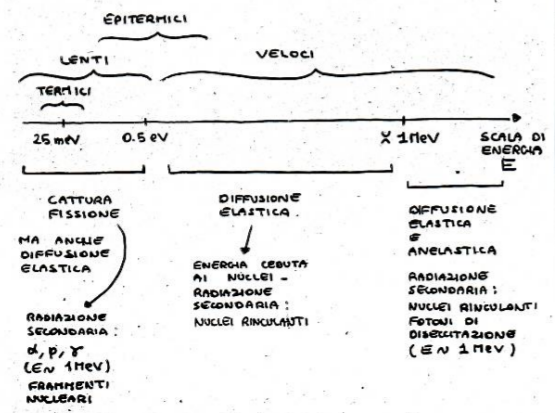
\includegraphics[scale=0.8]{./Immagini/InterazioneNeutroni.png}
\caption{Interazioni dei neutroni}
\end{center}
\end{figure}
Posta $\sigma_D$, $\sigma_C$, $\sigma_F$ la sezione d'urto dei due processi, allora la sezione d'urto totale risulta:
\begin{equation*}
\Sigma = N \, (\sigma_D + \sigma_C + \sigma_F)
\end{equation*}
con $N$ numero di nuclei per unit\`a di volume, per cui un fascio di $n_0$ neutroni seguir\`a la seguente legge:
\begin{equation*}
n(x) = n_0 \, e^{-\Sigma \, x}
\end{equation*}
Infine si definisce il libero cammino medio:
\begin{equation*}
\lambda = \Sigma^{-1}
\end{equation*}
per i neutroni veloci nell'ordine della decina di centimetri, per i lenti \`e nel centimetro.